\documentclass[a4paper, 11pt]{article}

\usepackage{geometry}
\geometry{a4paper,left=30mm,right=30mm, top=35mm, bottom=30mm}

\usepackage[ngerman]{babel}
\usepackage[utf8]{inputenc} 
\usepackage[T1]{fontenc}
\usepackage{algorithm}
\usepackage{amsmath}
\usepackage{amssymb}
\usepackage{amsthm}
\usepackage{enumerate}
\usepackage{array}
\usepackage{wasysym}
\usepackage{fancyhdr}
\usepackage{graphicx}
\usepackage{hyperref}
\usepackage{tabularx}
\usepackage {tikz}
\usetikzlibrary {positioning}
%\usepackage {xcolor}
\definecolor {processblue}{cmyk}{0.96,0,0,0}
\usepackage{latexsym}
\usepackage{lastpage} % Seitenzahlen
%\usepackage{MNsymbol}
\pagestyle{fancy}
\usepackage[noend]{algpseudocode}
\usepackage{caption}
\usepackage{amsmath}
\usepackage{tikz}
\usetikzlibrary{arrows}
\usepackage{tabularx} %schöne tabellen
\parindent0pt %einrücken verhindern
\bibliographystyle{unsrt}

\usepackage{polynom}
\cfoot{\thepage  \ / \pageref{LastPage}}

% % % % % % % % % % % % % % % % % % % % % % % %
% % % % % % % % % % % % % % % % % % % % % % % %
\newcommand{\modullang}{BAs}
\newcommand{\semester}{SoSe 2018}
\newcommand{\modul}{BA}
\newcommand{\blatt}{}
\newcommand{\tutorium}{Mi 16-18 Uhr}
\newcommand{\tutor}{}
\newcommand{\datum}{\today}
\renewcommand{\proofname}{Proof}
% % % % % % % % % % % % % % % % % % % % % % % %
% % % % % % % % % % % % % % % % % % % % % % % %

\begin{document} 
	
	%%% Kopfzeile linker Bereich
	%      gerade Seite   ungerade Seite
	\rhead[ \leftmark   ]{\textbf{}}
	%%% Kopfzeile mittlerer Bereich
	%      gerade Seite   ungerade Seite
	\chead[\leftmark   ]{\leftmark{}}
	%%% Kopfzeile linker Bereich
	%      gerade Seite             ungerade Seite
	\lhead[\textbf{}]{\blatt}
	
	
	%-- Deckblatt --						      
	\thispagestyle{empty}
	\begin{center}
		
		\vspace*{1.4cm}
		{\LARGE \textbf{Technische Universität Berlin}}
		
		\vspace{0.5cm}
		
		{\large Notes\\[1mm]}

		
		
		\vspace{1.0cm}
		{\LARGE \textbf{BlUB}}\\
		\vspace*{1.0cm}
		
		
		%	Babak \\
		%	Frank \\
		%	Kristian \\
		%	Rodrigo \\
		Sascha Lange%, 349960
		
		
		
	\end{center}
	
	\renewcommand{\labelenumi}{\alph{enumi})}
	\renewcommand{\labelenumii}{(\roman{enumii})}
	\renewcommand{\labelenumiii}{\arabic{enumiii}.}
	\renewcommand{\contentsname}{Table of Contents}
	%\renewcommand{\labelenumii}{\textbf{-}}	
	%-- Eigentlicher Text --
	\newpage
	\newtheorem{Cor}{Corollary}
	\newtheorem{Theorem}{Theorem}
	\newtheorem{Def}{Definition}
	\newtheorem{Prop}{Proposition}
	\newtheorem{Lemma}{Lemma}
	\section*{Meta Blub}
	
	Let $\mathcal{S}$ denote state space and $\mathcal{A}$ denote action space. Let $\mathcal{I}=\{1,...,P\}$ be  the set of players and $\mathcal{P}=\{N_1,...,N_{P}\}$ the set of corresponding (neural network) function approximators, where $N_i : \mathcal{S} \mapsto \mathcal{A}$, $N_i(s) = a$, %$s\in\mathcal{S}, a\in\mathcal{A}$,
	corresponds to player $i$. \\
	
	%We say player $i$ agrees with player $p$ (on states $s,s'$), if $N_i(s) = N_i(s')$ and $N_p(s) = N_p(s')$. This inspires the following:
	%Intro was ist los wir spielen hanabi
	%stability raus nach unten
	%nach $C_p(s)$ kommt dass das weighting fehlt
	%dann definieren wir stability
	%und similarity
	%schreiben neuen classifier
	%und dann die architecture
	
	Playing with a new teammate $p$, the goal is to predict the action $a$ that $p$ will take, facing a new state $s$. Based on the pool $\mathcal{P}$ of pretrained agents, we will define the notion of $consistency$ of two states, that will help us building a simple classifier to do so.
	\begin{Def}[consistency] {For $s,s'\in\mathcal{S}$, let  }
		%{Let $p\in\mathcal{P}, s, s'\in\mathcal{S}$.}
		\begin{align*}
		consistency_{\mathcal{P}}(s,s') = \frac{1}{P}\cdot|\{ i \in\mathcal{P}: N_i(s) = N_i(s')\}|.
		\end{align*}
		An agent $i\in\mathcal{I}$ is said to be consistent in $(s,s')$, if $N_i(s) =	 N_i(s')$.
	\end{Def}
 	We now define a simple distance function, which we can minimize later, to predict an action that $p$ will take:
	\begin{Def}[Distance] {For $s,s'\in\mathcal{S}$, let  the distance be defined as}
	\begin{align*}
	d(s, s') = 1 - consisteny_{\mathcal{P}}(s,s').
	\end{align*}
	\end{Def}
	After having observed data $D = \{(s_1, a_1),...,(s_n,a_n)\}$ from a new teammate $p$, we can give the action classifier as 
	\begin{align*}
	C_p(s) = \underset{a}{argmin} \{ d(\tilde{s}, s): (\tilde{s}, a)\in D \}.
	\end{align*}
	So we guess as the action $p$ takes in $s$, the action $p$ took in the state $s_{i\leq n}$,  with maximum $consistency_{\mathcal{P}}(s_{i\leq n}, s)$. However the suggested distance, does not account for the fact, that some players in $\mathcal{I}$ are more likely similar\footnote{similar w.r.t to which states they consider consistent} to $p$, than others. When the consistency voting happens, we would like to give those agents more weight than others. Therefore, we introduce the following notion on the observed data $D$:
	\begin{Def}[agreement] {For $s,s'\in\mathcal{S}, i,p\in\mathcal{P}$, let  }
		\begin{align*}
		agreement_D(i,p) =  \frac{2}{n(n-1)}\cdot|\{ (s,s')\in D\times D: N_i(s) = N_i(s') \text{ and } N_p(s) = N_p(s')\}|.
		\end{align*}
		%%Agent $i$ $agrees$ with $p$ on $(s,s')$, if $N_i(s) = N_i(s') \text{ and } N_p(s) = N_p(s')$
	\end{Def}
	The agreement of two agents $i,p$ is higher, the more pairs $(s,s')\in D$ exist, that $i$ and $p$ are both consistent on. Under the assumption, that this implies the agents are more likely to perform the same actions in new states, we now define p-similarity of two states, as a weighted version of consistency:
	

%It is beneficial however, to weight $d(\tilde{s},s)$ by $stability_p(\tilde{s},s)$ the obtain a $similarity$ of two states, relative to our teammate (for reasons I explained on slack).
	
	\begin{Def}[p-similarity] {For $s,s'\in\mathcal{S},i,p\in\mathcal{P}$, let  }
		\begin{align}
			similarity_p(s,s') = \frac{1}{P}\sum \{agreement_D(i,p)\in\mathbb{R}: i \text{ is consistent in } (s,s') \}.
		\end{align}
	\end{Def}
	
	
	
	
	
	Let $C_{\theta}$ denote our meta classifier. We want to learn $\theta=\theta_0$, such that
	\begin{itemize}
		\item after small number L of gradient steps on data $D$ from agent $A$, to obtain $\theta_L$, the network $C_{\theta_L}$ performs well on predicting actions of $A$
	\end{itemize}
	So we obtain updated network params after $i\leq L$ steps on $D$ from $A$ by
	\begin{align*}
	\theta^A_i = \theta^A_{i-1} - \alpha \Delta_{\theta} \mathcal{L}_A(C_{\theta^A_{i-1}})
	\end{align*} for a \textbf{single} Task $A$, and thus the meta-objective becomes
	\begin{align*}
	\sum_{A \in POOL} \mathcal{L}_{P}(C^A_{\theta_L}) =: \mathcal{L}_{Meta}, 
	\end{align*} where $\mathcal{L}_{P}$ denotes the loss on the hold out set corresponding to $A$. Both $A$ and $P$ are agents, but $A$ denotes agents at training time and $P$ denotes agents at test time, indicating that players can be humans. Note however, that \textbf{the different notation simply denotes disjoint data, but from the same agent P=A}.
	
	Finally we have the outer loop update given by
	\begin{align*}
	\theta_0 = \theta_0 - \beta \Delta \mathcal{L}_{Meta}.
	\end{align*}
	
	Using the idea of incorporating implicit soft cluster assignment (see slack) into the learning process we may obtain for $C_\theta$ the following architecture:\\
	
	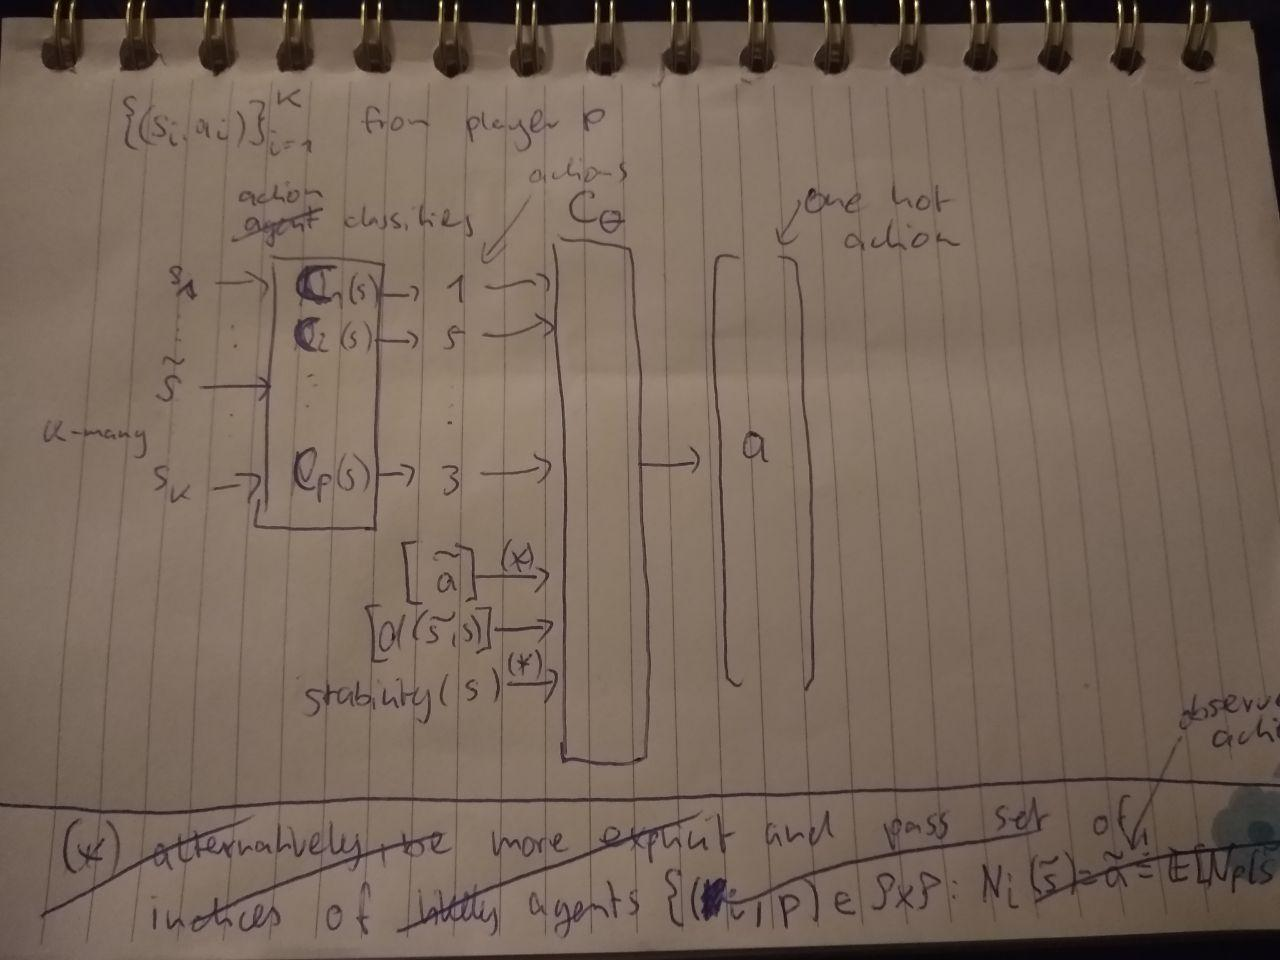
\includegraphics[scale=.5]{architecture}
	
	%When observing a new player $p$ and using the notion of stability of a state, we can try to estimate the relative skill of $p$, by computing $\frac{2}{P(P-1)}\cdot|\{ (N_i, p) \in\mathcal{N}\times\mathcal{N}: N_i(s) = E[N_p](s)\}=:D|$, where $E[N_p](s)$ will be observed through actual playing with $p$ and observing state action pairs $(s,a)$. Define the set of players $\bar{D} = \{ (N_i, p) \in\mathcal{N}\times\mathcal{N}: N_i(s) \neq E[N_p](s)\}$, for which a different action than $a$ has been predicted. The goal is, using meta-learning, to increase the weight of players in $D$ and decrease the weight of players in $\bar{D}$, to get a notion of similarity, that is relative to the player we want to predict actions for. \\
	%Let d(s, s') be given by the inverse $Agreement$ of $s$, and $s'$.
	%In order to be able to cast this into the MAML framework, we define the set of possibly infinite tasks to be set of possible teammates (for which we want to predict actions).
	%During training of the meta learner, we are trying to find out how to change for different possible teammates the weights (coming from $D$ and $\bar{D}$ each step) for similarity computation, such that predictions of actions using the ensemble of agent networks, will be most accurate.
	
	%Training:
	%will do this today
	
	
	
\end{document}

%Python’s default arguments are evaluated once when the function is defined, not each time the function is called (like it is in say, Ruby). This means that if you use a mutable default argument and mutate it, you will and have mutated that object for all future calls to the function as well. (https://docs.python-guide.org/writing/gotchas/)
